\setcounter{step}{0}
%------------------------------------------
% information doc
\subsection{Naan}
%------------------------------------------

\begin{ingredient}

%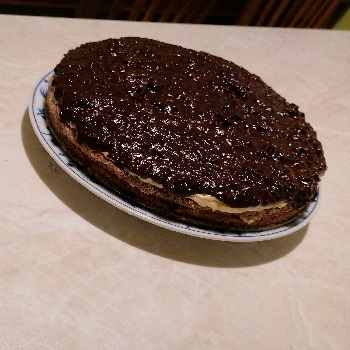
\includegraphics[height=5.5cm]{images/daim}
\def\portions{2}%
\textbf{{\normalsize Ingrediencie (\portions porcie):}}

%\vspace{0.5cm}
\begin{main}
	\item 260g hladká múka
	\item 2 KL kypriaci prášok
	\item 1/2 KL soľ
	\item 1 KL kryštálový cukor
	\item 150g biely jogurt
	\item 1 PL olivový olej
	\item 1-3 PL mlieko 
	\item 2 strúčiky cesnak
	\item 1/2 hrste koriander
	\item 1 KL maslo
\end{main}
\end{ingredient}
\begin{recipe}
\textbf{{\normalsize Príprava:}}
\begin{enumerate}
\item{Zmiešame múku s práškom do pečiva, soľou a cukrom. Všetko dobre premiešame.}
\item{Pridáme jogurt, olej, a lyžicu mlieka.}
\item{Všetko spracujeme do celistvého cesta, ak treba, pridáme ešte trochu mlieka.}
\item{Cesto premiestnime na pomúčenú pracovnú dosku, dobre ho prehnietime a rozdelíme na 2 až 4 časti.}
\item{Cesnak nakrájame na tenké plátky a koriander nasekáme na drobno.}
\item{Z každej časti cesta vyvaľkáme tenkú placku.}
\item{Na dosku položíme plátky cesnaku, nasekaný koriander a preložíme ich plackou, zvlaľkáme dokopy.}	
\item{Pečieme na suchej, rozpálenej panvici asi 3 minúty z každej strany.}
\item{Pomastíme maslom.}
\end{enumerate}

\end{recipe}

\begin{notes}

\end{notes}	
\clearpage